\begin{figure}[h]
	\centering
	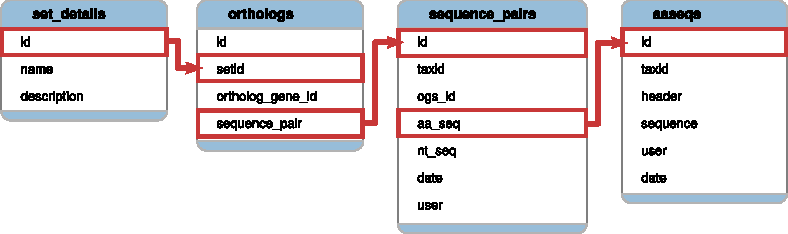
\includegraphics{img/db-orthoset.pdf}
	\caption[Database table connections for a given ortholog set]{
		\pname database structure for a given ortholog set. Each rounded rectangle
		represents a table with named columns. The red path delineates the
		\code{JOIN} query structure that returns all amino acid sequences (stored in
		the table ``aaseqs'') that belong to a given ortholog set. Ortholog set
		information is stored in the table ``set\_details''.
	}
	\label{fig:db-orthoset}
\end{figure}
